\paragraph{Definition:} Causal reasoning refers to the ability to infer, analyze, understand, and explain the causal relationships between events and actions. 
Tasks in this domain can be classified into the following parts:

\begin{enumerate}
    \item \textbf{Causal discovery}:  Identifying causal relationships between two or more events. 
    This typically answers questions like: Is event A the cause of event B?

    \item \textbf{Effect inference}:   Once the causes of an outcome are known, it is important to understand how much those causes contribute to the outcome.
    In other words, one seeks to estimate the magnitude of the cause’s impact on the current result.\
    
    \item \textbf{Attribution}: The goal of this task is to identify which cause is the main driver behind a specific change.
    \item \textbf{Judgment}: This is an extension of Attribution, where rewards or blame are assigned to actions based on other causal relationships
    In other words, it makes decisions based on causal relationships. 
\end{enumerate}

\begin{figure}
    \centering
    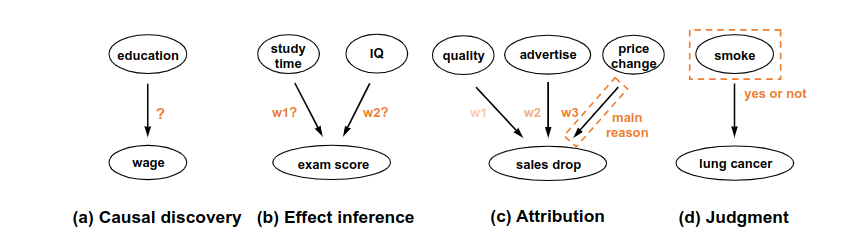
\includegraphics[width=0.9\textwidth]{Figs/causal_graph.png}
    \caption{Causal graph describe the four tasks of Causal Reasoning}
    \label{fig:causal_graph}
\end{figure}


To represent these relationships, causal graphs (causal networks) are used, which are graphs depicting the causal relationships between variables or events. 
In such graphs, variables or events are represented by nodes, and the causal relationships between them are represented by directed arrows. 
Figure \ref{fig:causal_graph} uses a causal graph to describe the four tasks mentioned above


\subsubsection{Counterfactual Reasoning}

Counterfactual \cite{li2023counterfactual} is introduced as a method to assess the reasoning and understanding abilities of large language models in hypothetical scenarios. 
In this context, counterfactuals are defined as things that are false in the real world but true in a hypothesis
Since most large language models are trained on human knowledge or real-world knowledge, having the model reason based on hypothetical knowledge 
(which it may not have learned or known) can expand and evaluate its reasoning ability, forcing it to make unusual conclusions or predictions


\paragraph{Formula:} Let x $\in$ X be the input, where X represents knowledge $w$ in the worlds W, to produce an output $y \in Y$. This defines a function $f$ that perfomrs
a mapping: X $\rightarrow$ Y. The counterfactual reasoning is defined as the function $f_{cf}$: X $\times$ W $\rightarrow$ Y. Assuming that $h$ approximates functions $f_w$, where w 
can be real world or counterfactual world, a large language model implementing $f_w$ can be described as follows: 

\[
h(f, w, x) = argmax_{y \in Y} P_{LM}(y' | prompt_f(f, x), prompt_w(w))
\]

where $prompt_f$ and $prompt_w$ are the prompts for the function $f$. 


The study \cite{wu2023reasoning} employs counterfactual reasoning to evaluate the abstract reasoning capabilities of large language models (LLMs). 
The paper proposes a framework consisting of 11 hypothetical tasks designed to assess the reasoning abilities of LLMs. 
The performance of models such as GPT-4, Claude, and PaLM-2 is compared across tasks in both default worlds and counterfactual worlds.
The findings indicate that current models can handle abstract tasks to a certain extent. However, their capabilities are heavily dependent on narrow, context-specific settings, 
highlighting the limitations in generalizing abstract reasoning across diverse context. 

Additionally, the study \cite{li2023counterfactual} investigates how pretrained language models (PLMs) handle counterfactual conditions. 
The primary goal of the research is to assess whether PLMs can distinguish between hypothetical situations and real-world scenarios
The study concludes that when faced with counterfactual situations, PLMs often generate text that contradicts established real-world knowledge
. Furthermore, PLMs tend to prioritize closer contextual information over more general knowledge when reasoning in hypothetical scenarios. This indicates that language models are not only influenced 
y the world knowledge they have learned but are also affected by the linguistic structure and the specific context of the scenarios presented to them.

